\documentclass[a4paper,10pt]{article}
\usepackage{graphicx}

%opening
\title{\textbf{Studio di un Modello di Integrazione (??)}}
\author{Jacopo Baldassarri (Laurea Magistrale in Informatica)\\Andrea Blasco (Dottorando in Economia)\\Elisa Omodei (Laurea Magistrale in Fisica)}

\begin{document}

\maketitle

%\begin{abstract}
%\end{abstract}

\section{Descrizione del Modello}
Da scrivere

\newpage

\section{Parte Informatica}
Il nostro progetto \`e stato implementato utilizzando il linguaggio C++, con l'utilizzo delle librerie fltk sotto ambiente Linux. Sono stati
utilizzati gli editor Kate e Gedit per la scrittura del codice, il programma Gnuplot per la realizzazione delle figure e l'ambiente Kile per
la stesura della relazione.\\
Abbiamo deciso 
di suddividere il codice in due parti distinte, una parte testuale in cui non vi \`e nessun tipo di visualizzazione del modello, che ci 
permettesse di fare delle simulazioni molto velocemente; ed una parte grafica nel quale viene visualizzata una vista del modello e dove \`e 
possibile modificare i vari parametri di simulazione.
\subsection{Grafica}
La parte grafica \`e stata realizzata mediante l'utilizzo delle librerie fltk, \`e stato creato un main .cxx con l'inizializzazione di tutti 
gli elementi grafici della nostra interfaccia, quali slider, bottoni per il controllo di sequenza ecc. e delle classi per l'implementazione
del  nostro modello.\\
Nella classe simulationGrid.cpp viene realizzata la parte grafica, in cui vengono disegnati tutti i vari agenti e i vari link fra di essi, \`e 
la classe che si occupa anche della reinizializzazione grafica nel caso in cui vengano modificati i parametri del modello.\\
Il compito della realizzazione vera e propria del modello \`e affidata alla classe model.cpp nel quale vengono inizializzate tutte le strutture 
dati necessarie alla simulazione, mediate l'utilizzo di malloc per allocazione della memoria, viene riservato spazio per le matrici nel quale 
andranno ad essere inseriti i dati degli agenti e le loro amicizie. Inoltre la classe si occupa dell'aggiornamento delle matrici, calcolando ad 
ogni passo di iterazione gli opportuni valori di correlazione e di amicizie che vengono inseriti nelle strutture dati.\\
Vi \`e inoltre una classe widgetWindow.cpp che si occupa di creare e di aggiungere all'interfaccia grafica delle  finestre di statistiche sul
quale verranno visualizzati dei valori interessanti del modello che vengono monitorati a run time durante la simulazione.\\
Abbiamo inoltre una superclasse glStats.cpp che rappresenta una generica statistica da visualizzare in una delle sotto-finestre, nel quale 
vengono impostati tutti i parametri di visualizzazione.\\
Sono invece le tre sottoclassi capitalVariation.cpp, clusteringStats.cpp e degreeStats.cpp che implementano la visualizzazione delle statistiche del
modello che vengono disegnate a run time nelle sotto-finestre.\\
Abbiamo infine la classe gui\_controls.cpp in cui sono realizzate tutte le funzioni per le slider dell'interfaccia grafica e per i pulsanti di 
controllo  di sequenza, quali play, pause e stop.\\
Nell'interfaccia grafica, ogni agente viene rappresentato da un cerchietto, tanto pi\`u grande quanto \`e maggiore il suo numero diamicizie
e con un colore che cambia in base al suo codice genetico.\\
\`E stato inoltre realizzato un algoritmo di Spring Embedding per la disposizione sulla griglia, cos\`i che agenti con una correlazione
maggiore siano disposti pi\`u vicini fra loro.

\begin{figure}[!ht]
\begin{center}
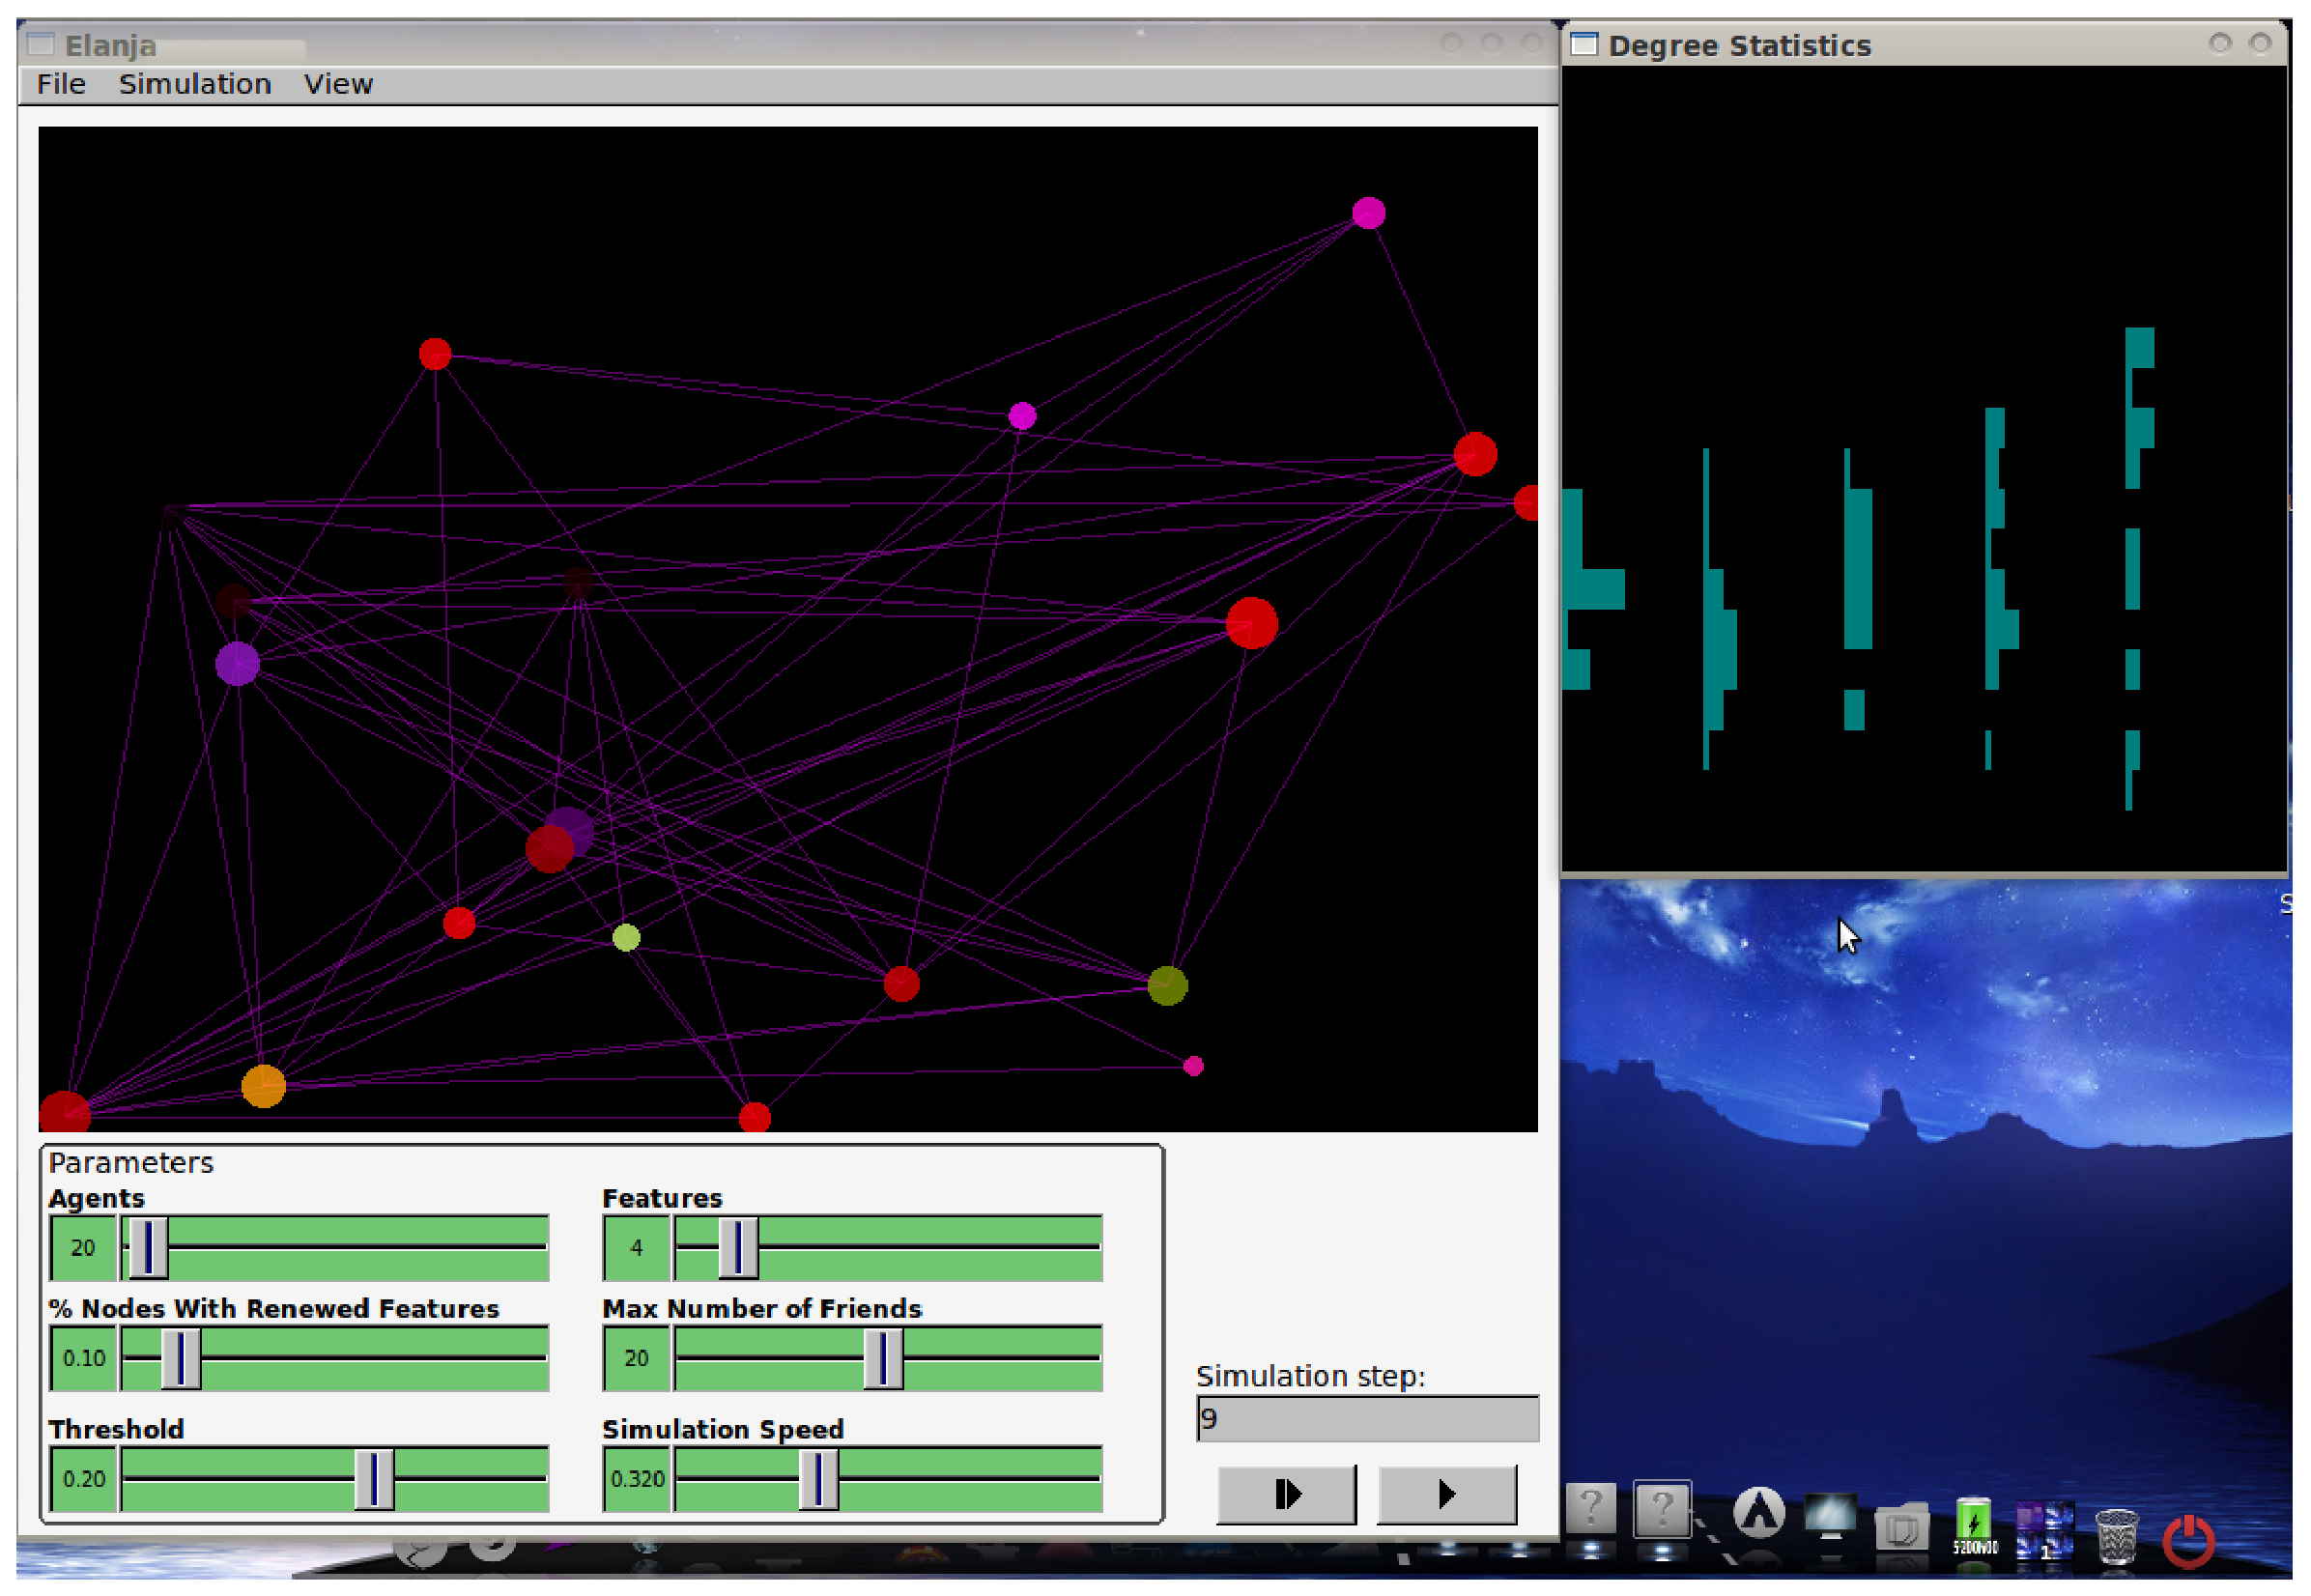
\includegraphics[width=\textwidth]{GUI.eps}
\end{center}
\caption{Interfaccia grafica e statistica delle amicizie}
\end{figure}

\subsection{Testuale}
Nella parte testuale ovviamente le classi che abbiamo realizzato sono notevolmente ridotte, infatti non sono pi\`u necessarie tutte le parti
di visualizzazione del modello e delle statistiche.\\
Abbiamo in questa parte solo due classi, la classe elanja.cpp che \`e il main del progetto testuale e che si occupa di eseguire i passi di 
simulazione e di stampare delle statistiche in dei file specificati cos\`i che queste possano essere elaborate in un secondo momento. Essa si 
occupa anche di inizializzare i parametri del modello, o in base a dei parametri di default, contenuti nel file const.h, oppure in base ai
parametri che l'utente fornisce al momento dell'invocazione dell'eseguibile del progetto da terminale. Infatti in questo frangente \`e 
possibile specificare al momento dell'esecuzione quali sono i parametri con il quale fare le simulazioni; mentre nella sezione grafica questo 
non \`e supportato, dato che \`e possibile farlo a run time mediante l'interfaccia grafica

\begin{figure}[!ht]
\begin{center}
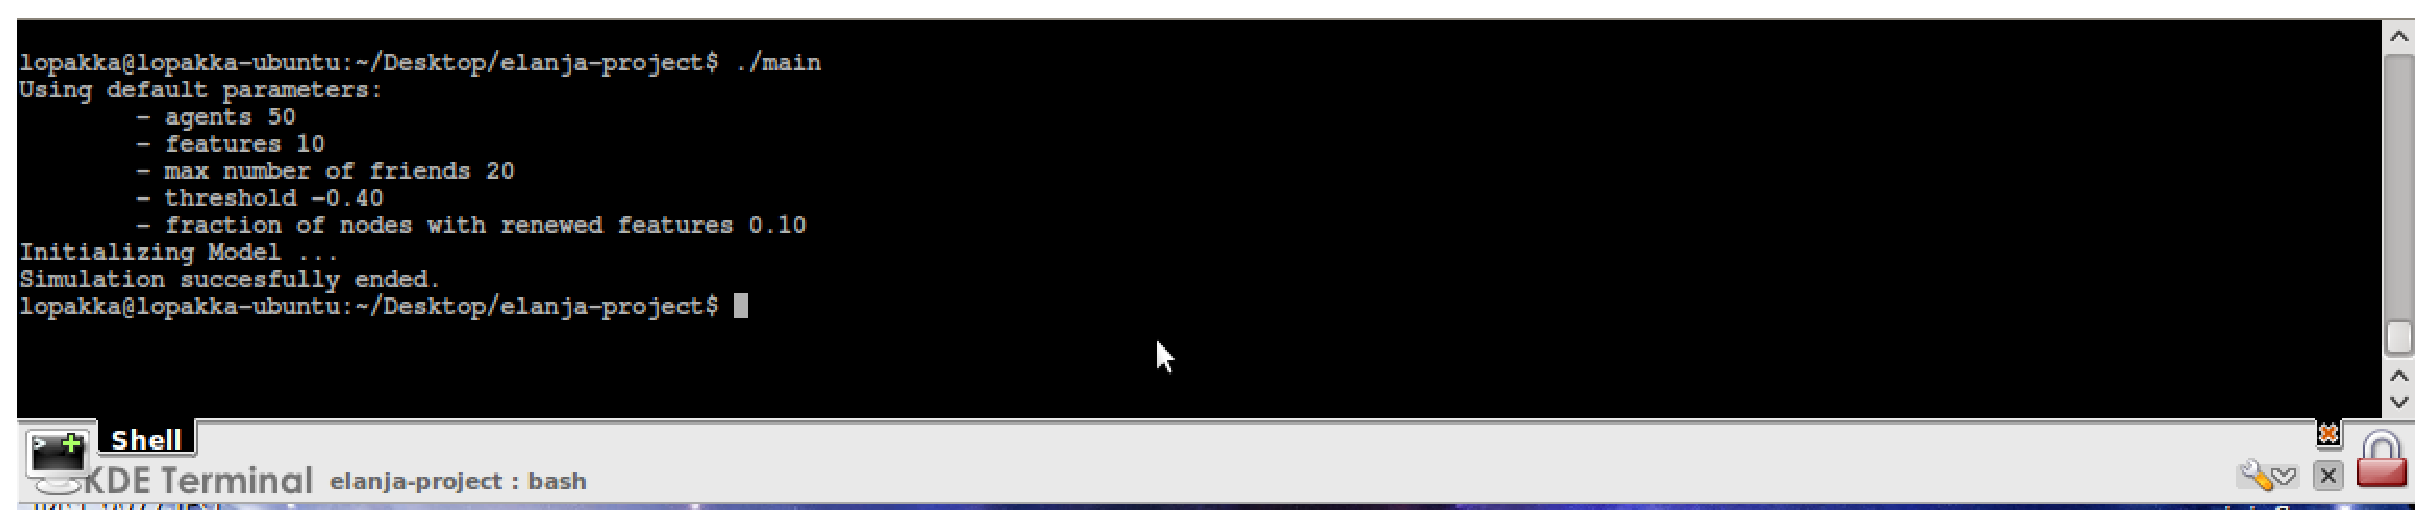
\includegraphics[width=\textwidth]{Text.eps}
\end{center}
\caption{Versione testuale della simulazione}
\end{figure}

\newpage

\section{Risultati Numerici}
\subsection{Caso Statico}
Abbiamo innanzitutto studiato il modello nel caso statico, cio\`{e} il caso in cui $\rho = 0$ e quindi non avviene una reinizializzazione di una parte delle features ad ogni step.
I parametri fissi sono:
\begin{itemize}
\item numero di agenti: N = 1000;
\item numero massimo di link per agente: $\tau = 20$.
\end{itemize}
I parametri che abbiamo fatto variare sono invece:
\begin{itemize}
\item threhsold, da $-0.8$ a $0.8$ a passi di $0.2$;
\item numero di feature, da 5 a 30 a passi di 5.
\end{itemize}
Per ognuno dei 36 casi (9 variazioni della threshold per 6 variazioni del numero di features) abbiamo eseguito 20 simulazioni.

\begin{figure}[!ht]
\begin{center}
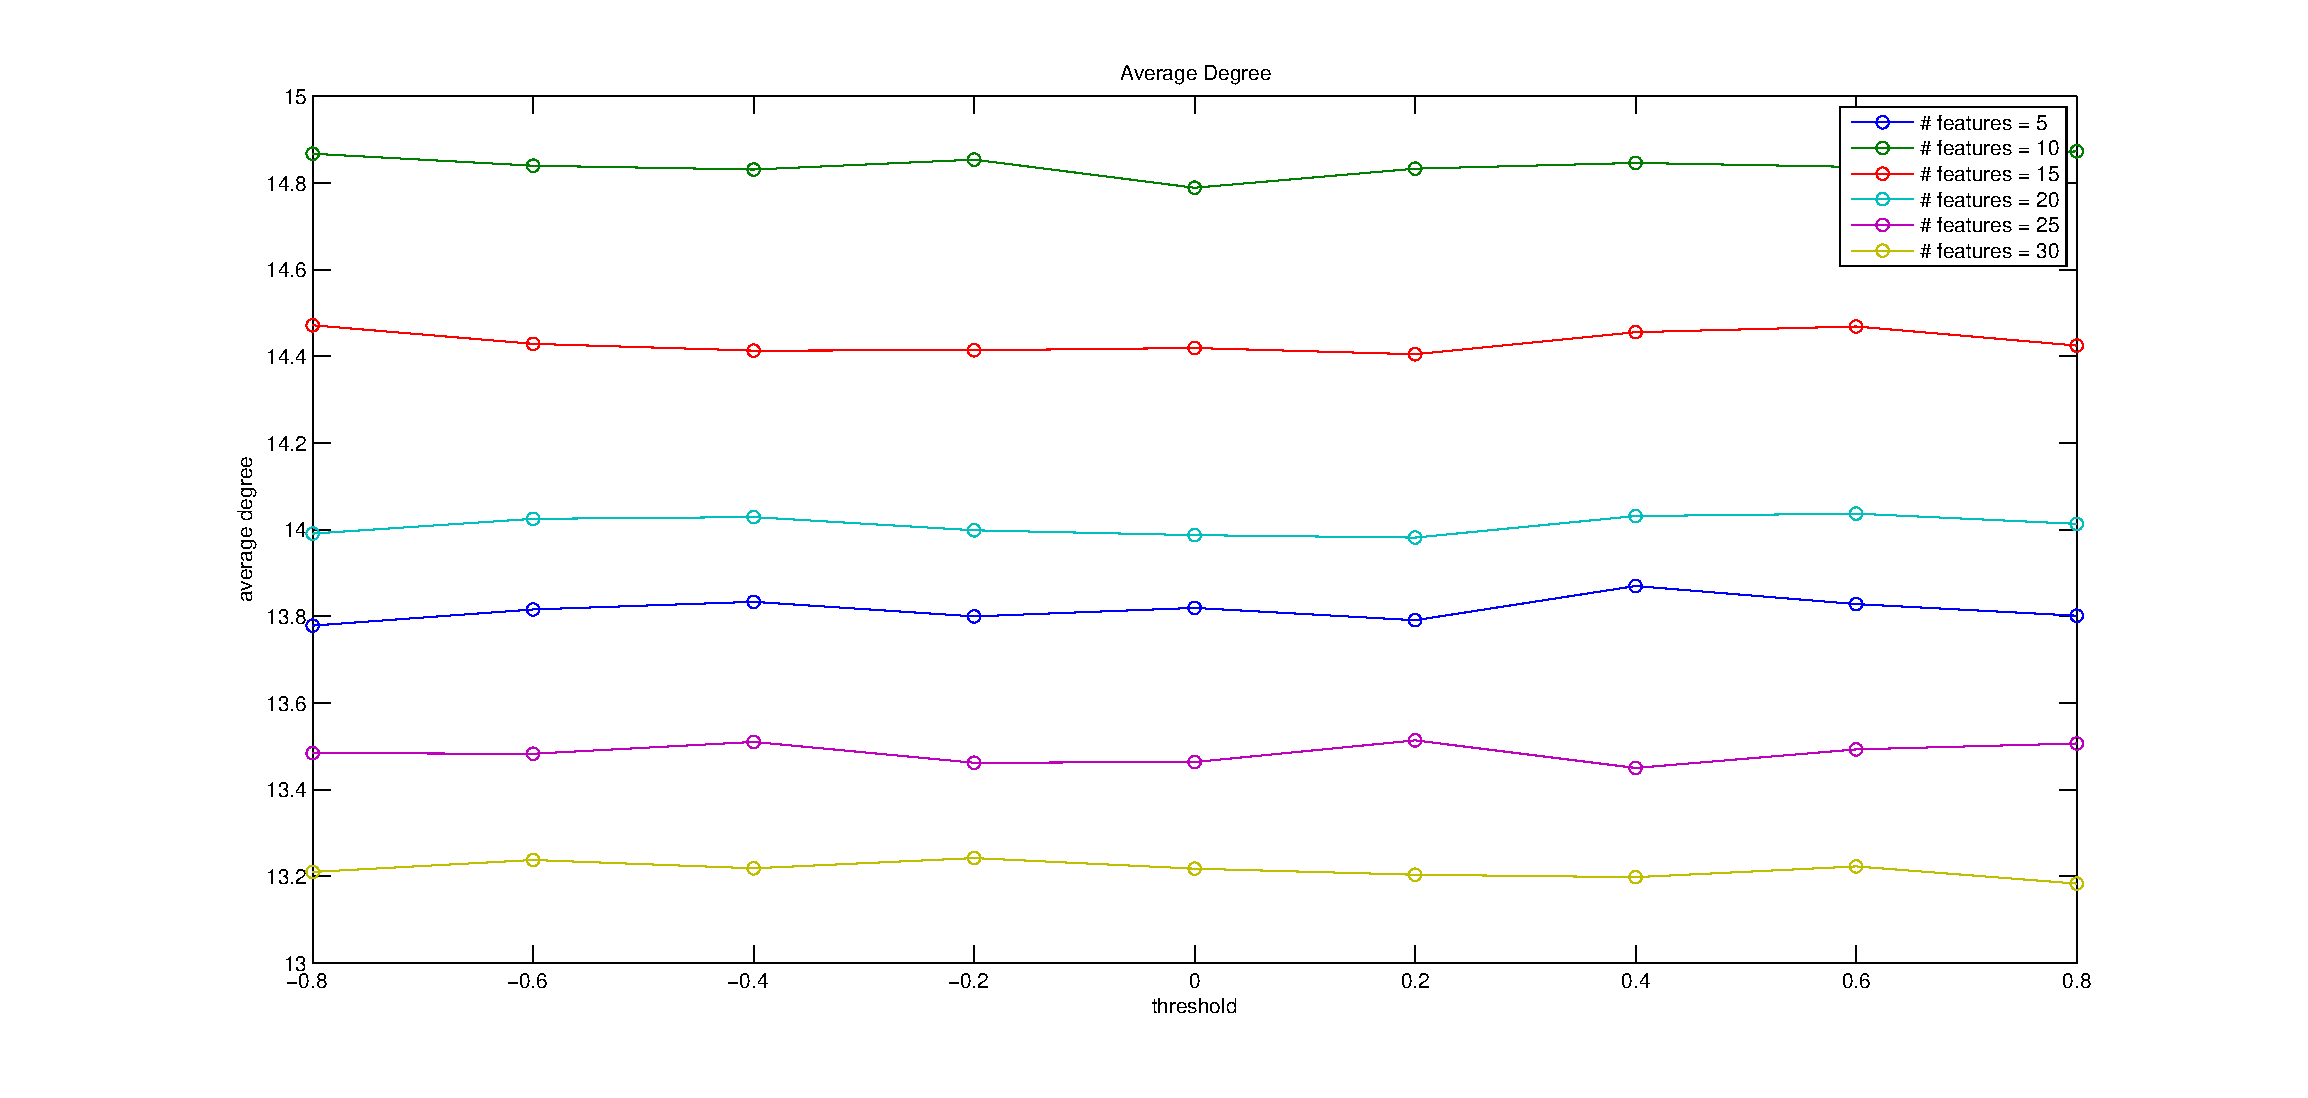
\includegraphics[width=\textwidth]{AverageDegreeThreshold.eps}
\end{center}
\caption{Connettivit\`{a} media al variare della threshold, tenendo fisso il numero di features}
\label{2.1.1}
\end{figure}

\begin{figure}[!ht]
\begin{center}
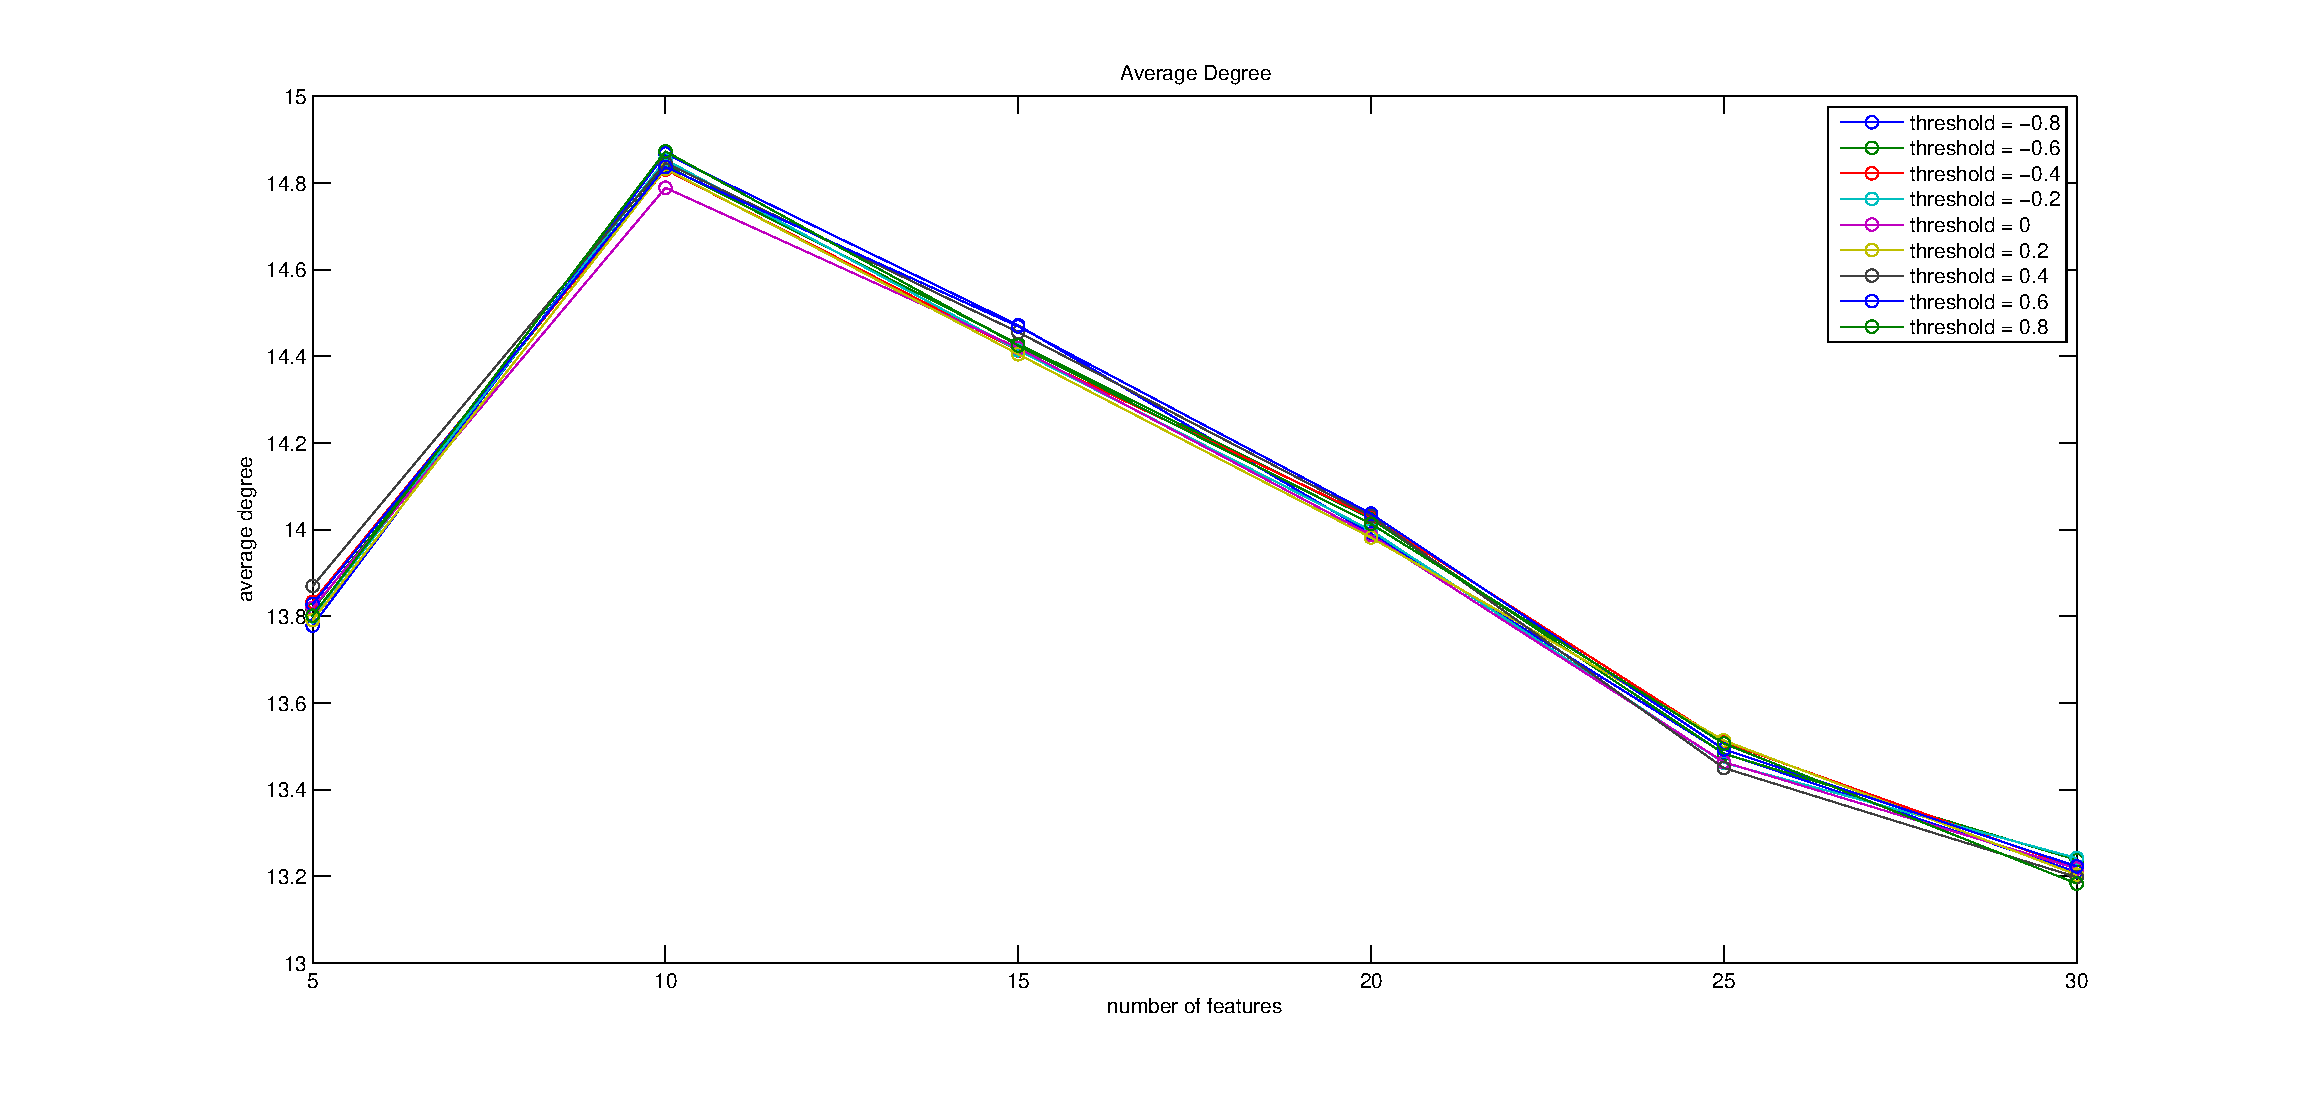
\includegraphics[width=\textwidth]{AverageDegreeFeatures.eps}
\end{center}
\caption{Connettivit\`{a} media al variare del numero di features, tenendo fissa la threshold}
\label{2.1.2}
\end{figure}
In Figura~\ref{2.1.1} \`{e} riportata la connettivit\`{a} media degli agenti al variare della threshold, tenendo fisso il numero di features; in Figura~\ref{2.1.2} \`{e} riportata nuovamente la connettivit\`{a} media, ma questa volta tenendo fissa la threshold e variando il numero di features.
\\Possiamo osservare come la connettivit\`{a} media non mostra alcuna dipendenza dal valore della threshold, mentre varia significativamente al variare del numero di features. 
L'andamento della connettivit\`{a} media al variare del numero di feature presenta un massimo per numero di features pari a 10 e poi decresce linearmente.
\\\\Per capire come mai la connettivit\`{a} media non varia al variare della threhsold, abbiamo analizzato come varia il tvalue medio al variare della threhsold e del numero di features. Infatti \`{e} il tvalue il valore effettivo che discrimina la formazione o meno di link.

\begin{figure}[!ht]
\begin{center}
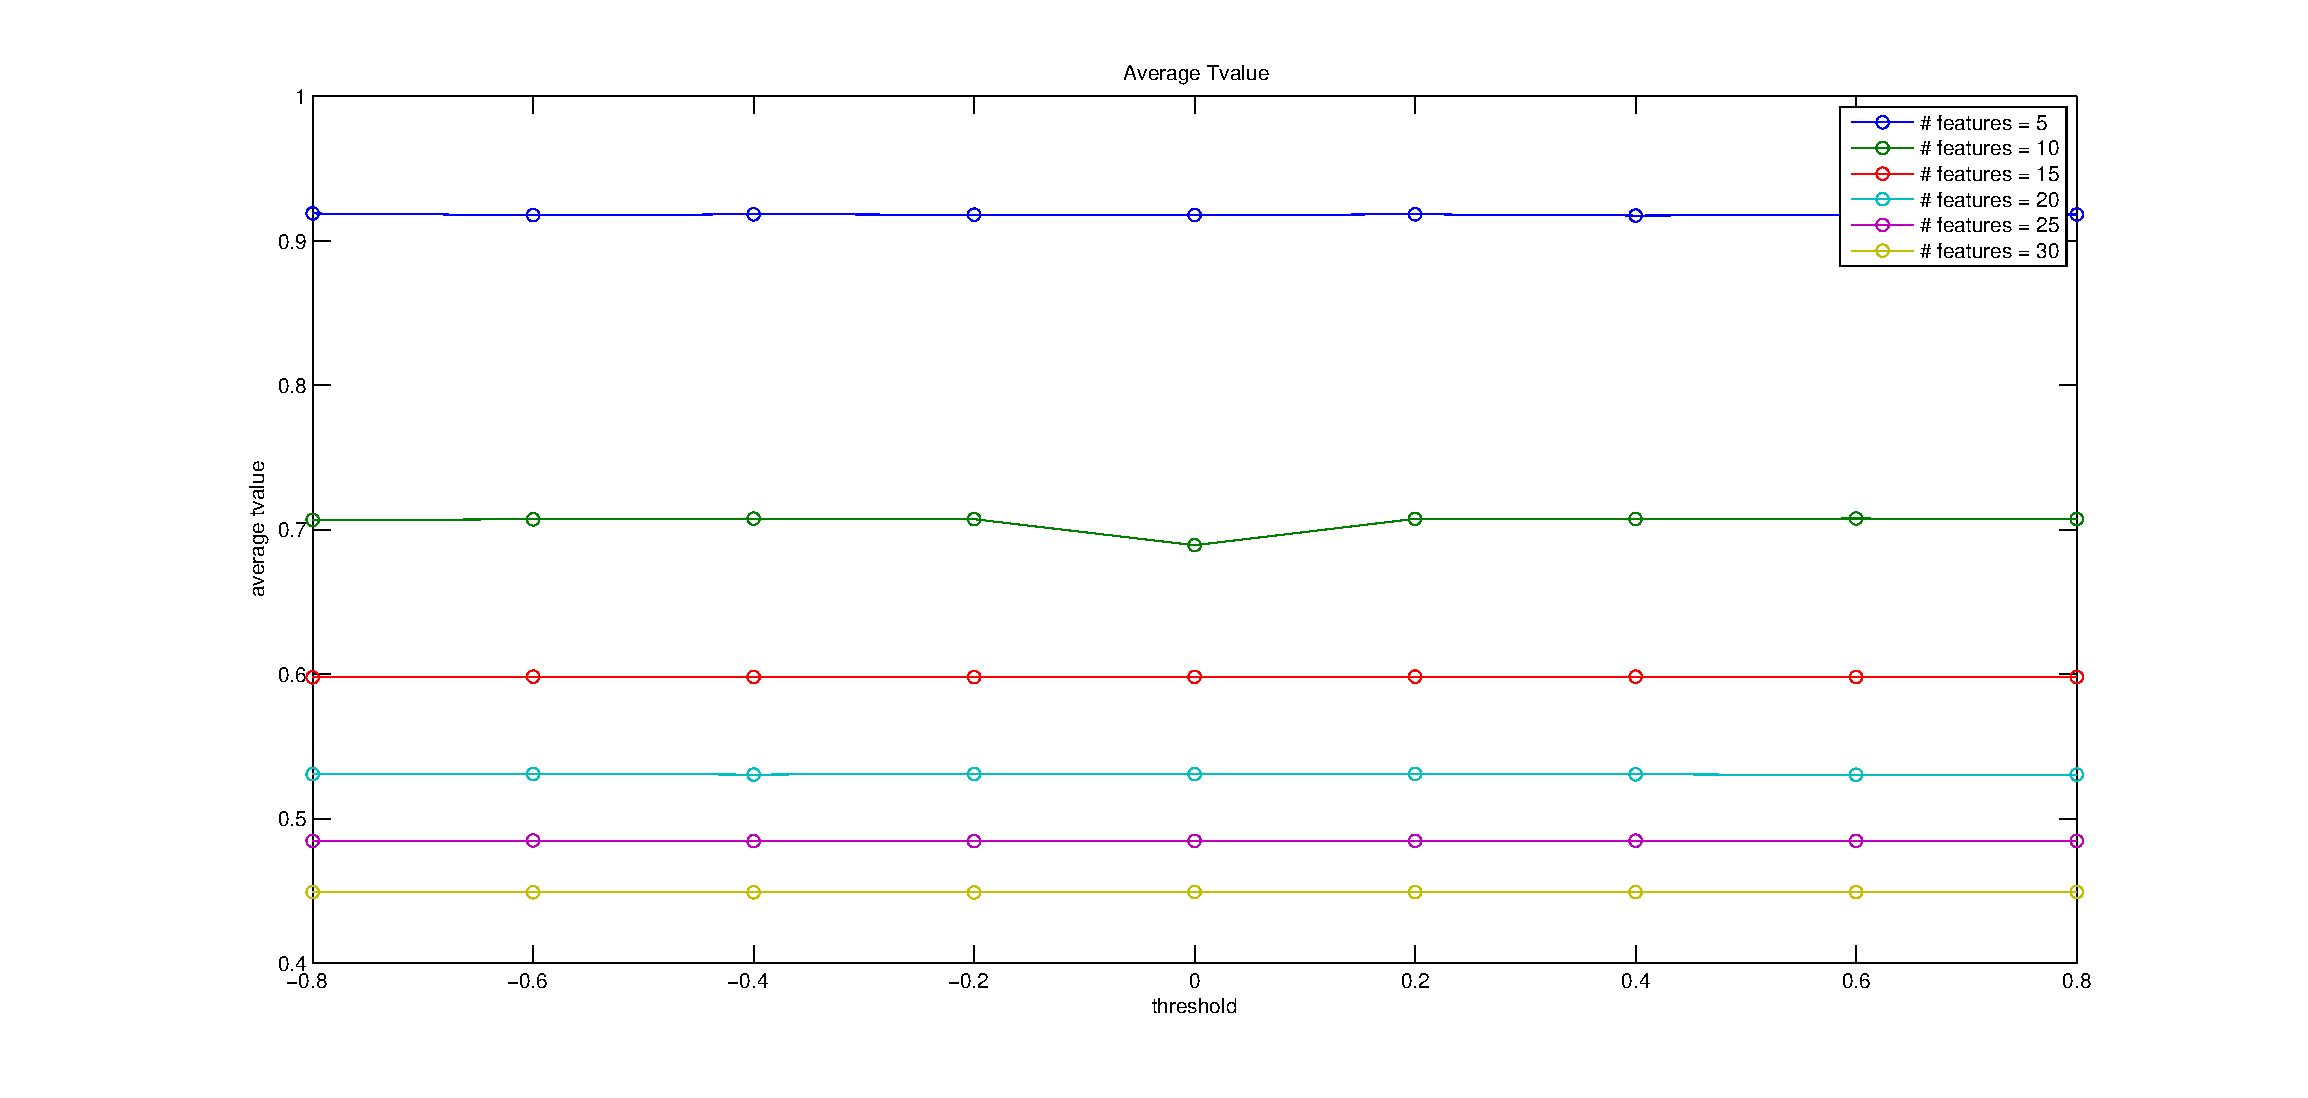
\includegraphics[width=\textwidth]{AverageTvalueThreshold.eps}
\end{center}
\caption{Tvalue medio al variare della threshold, tenendo fisso il numero di features}
\label{2.1.3}
\end{figure}

\begin{figure}[!ht]
\begin{center}
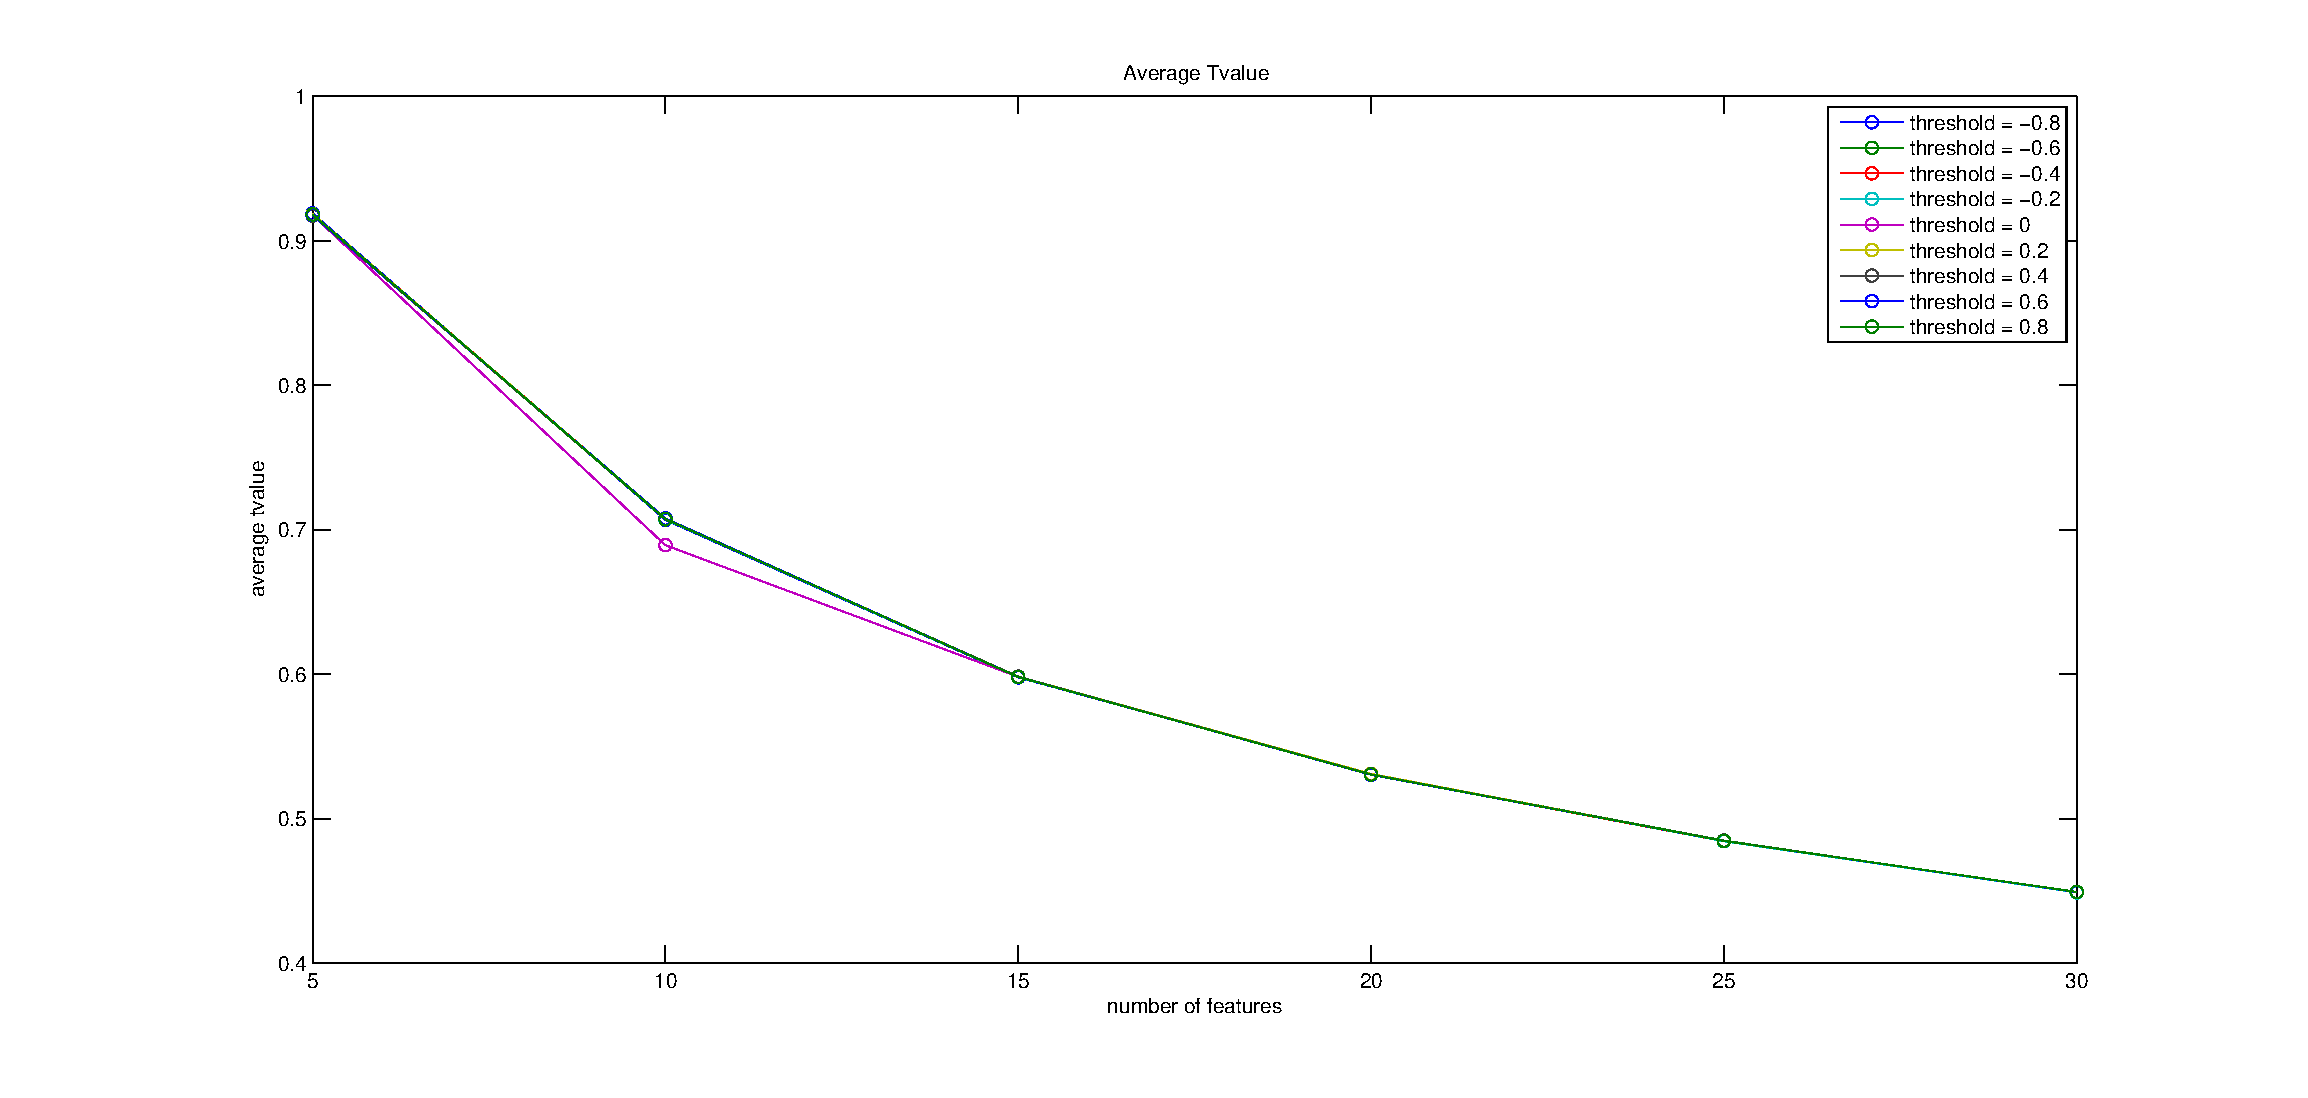
\includegraphics[width=\textwidth]{AverageTvalueFeatures.eps}
\end{center}
\caption{Tvalue medio al variare del numero di features, tenendo fissa la threshold}
\label{2.1.4}
\end{figure}

Osserviamo che anche il tvalue non presenta una dipendenza dal valore della threshold, ma presenta invece una forte dipendenza dal numero delle features.
Questo significa che, dato un valore della threhsold, per soddisfare il vicolo del numero massimo di link per agente, il sistema \`{e} costretto ad aumentare o diminuire il tvalue (ovvero il valore effettivo della threhsold), e il valore medio finale \`{e} costante per qualsiasi valore iniziale della threhsold, mentre varia fortemente al variare del numero di features.
\\Possiamo dunque concludere che il parametro caratterizzante del sistema \`{e} proprio il numero di features proprie di ogni agente, e non il valore iniziale assegnato alla threshold.
\\\\Per caratterizzare il sistema abbiamo poi studiato un altro parametro: la media e la varianza medie delle features di ciascun agente.

\begin{figure}[!ht]
\begin{center}
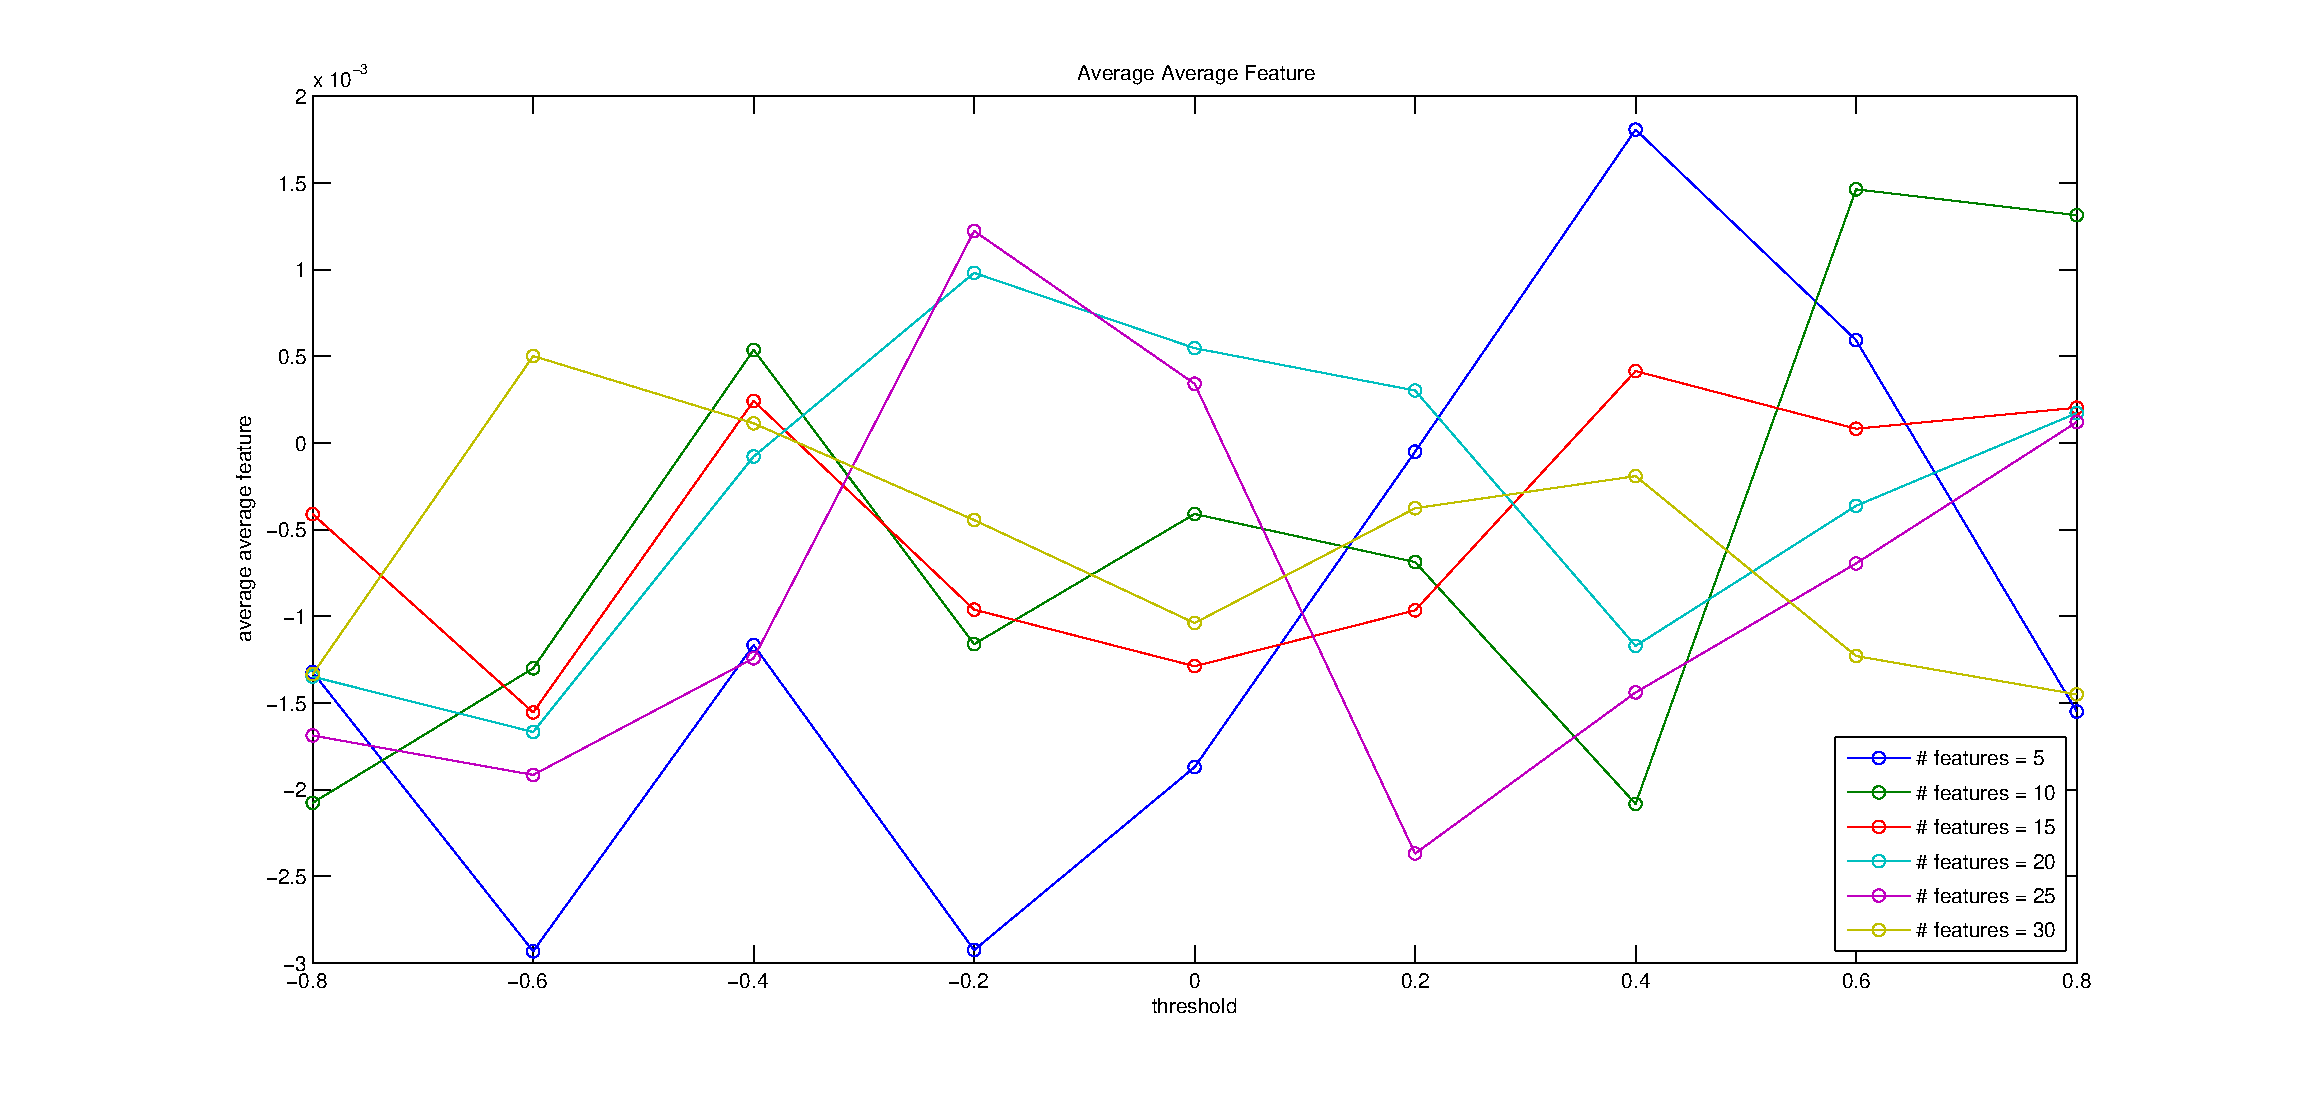
\includegraphics[width=\textwidth]{AverageAverageFeatureThreshold.eps}
\end{center}
\caption{Feature media media al variare della threshold, tenendo fisso il numero di features}
\label{2.1.5}
\end{figure}

\begin{figure}[!ht]
\begin{center}
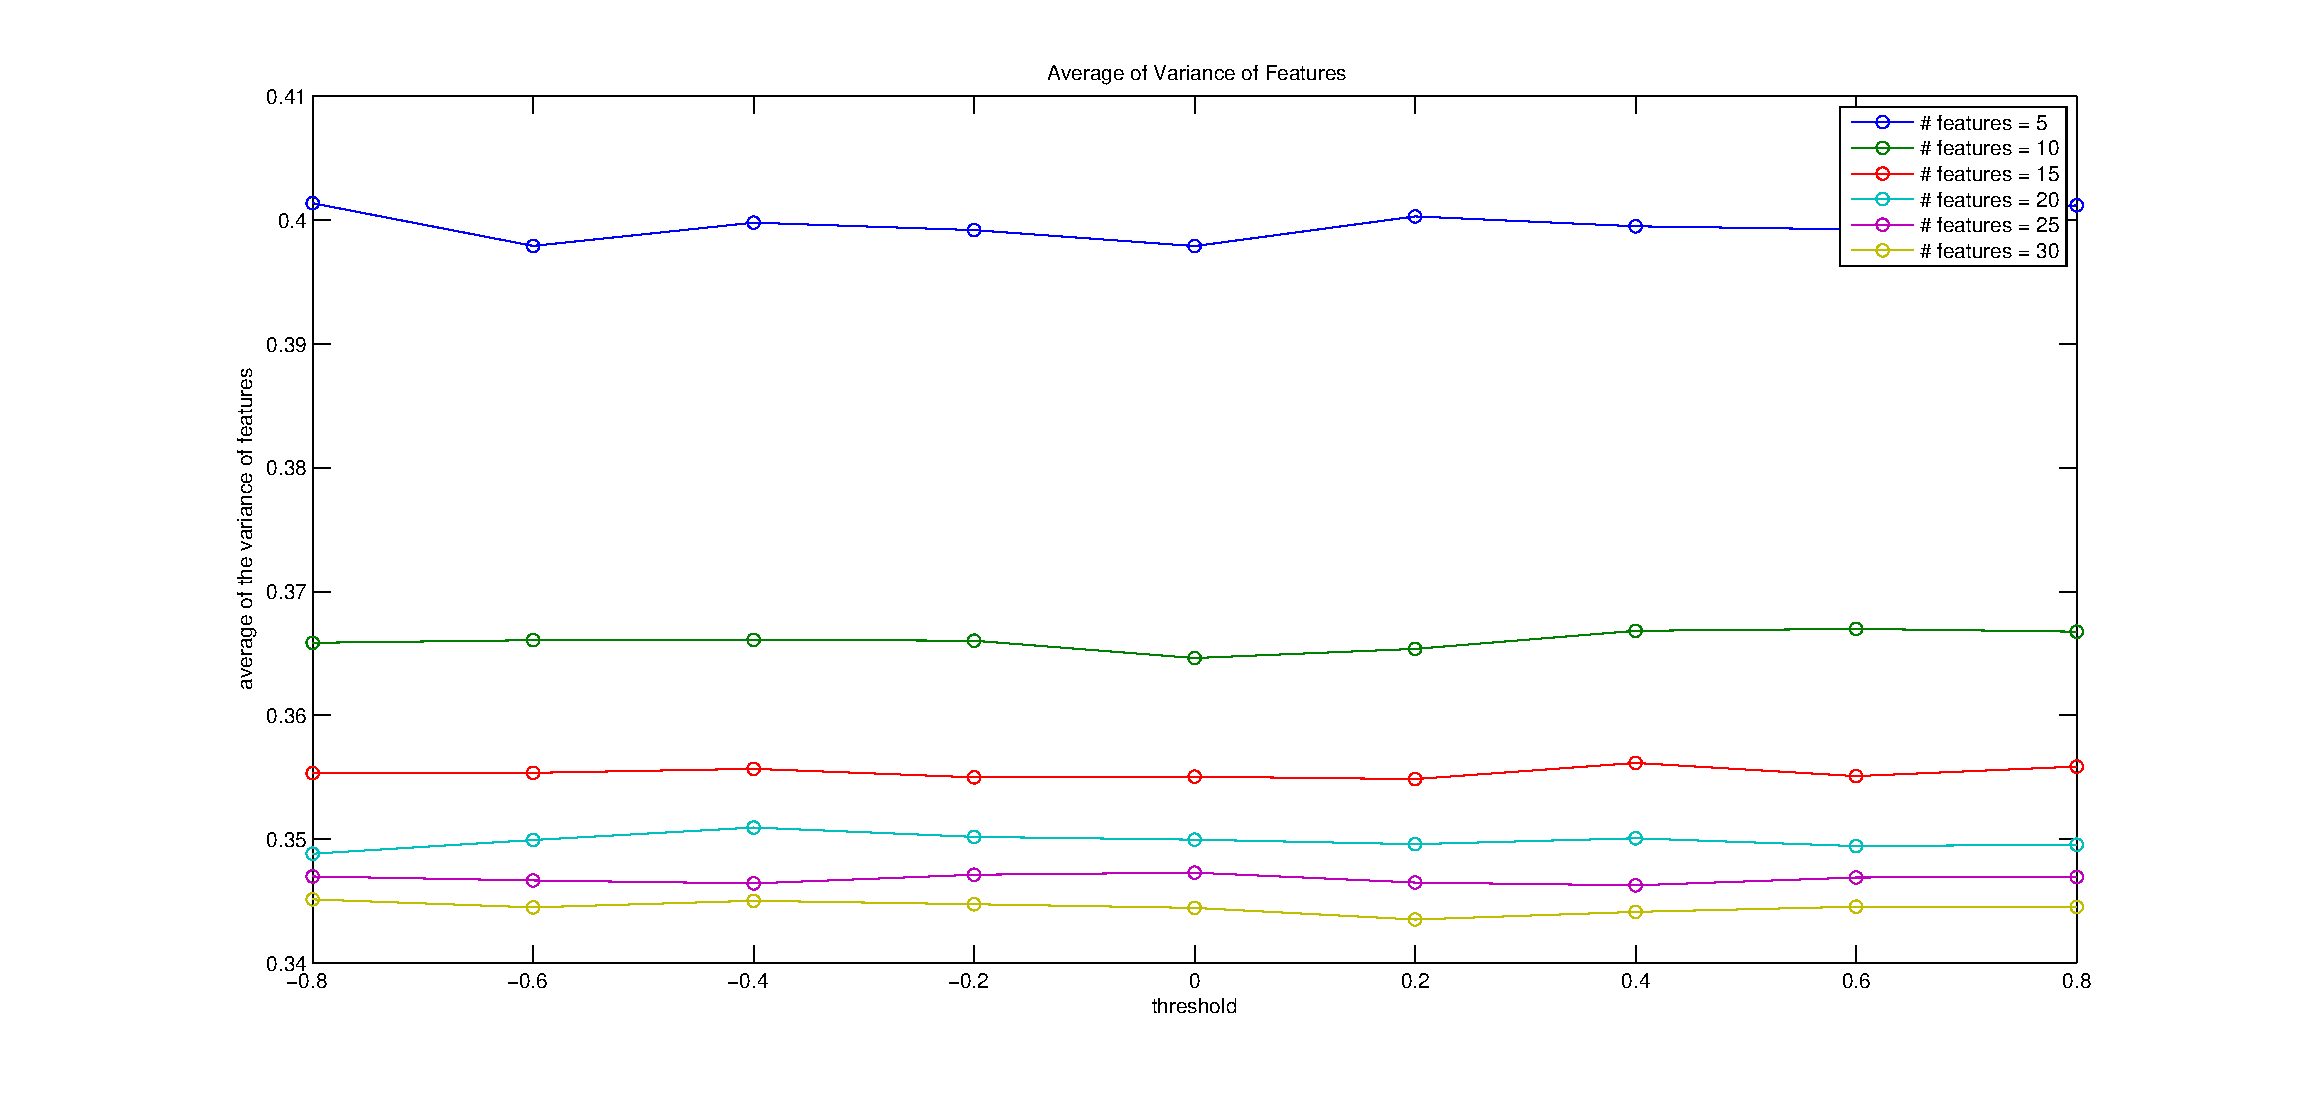
\includegraphics[width=\textwidth]{AveVarFeatThreshold.eps}
\end{center}
\caption{Varianza media delle features al variare della threshold, tenendo fisso il numero di features}
\label{2.1.6}
\end{figure}

\begin{figure}[!ht]
\begin{center}
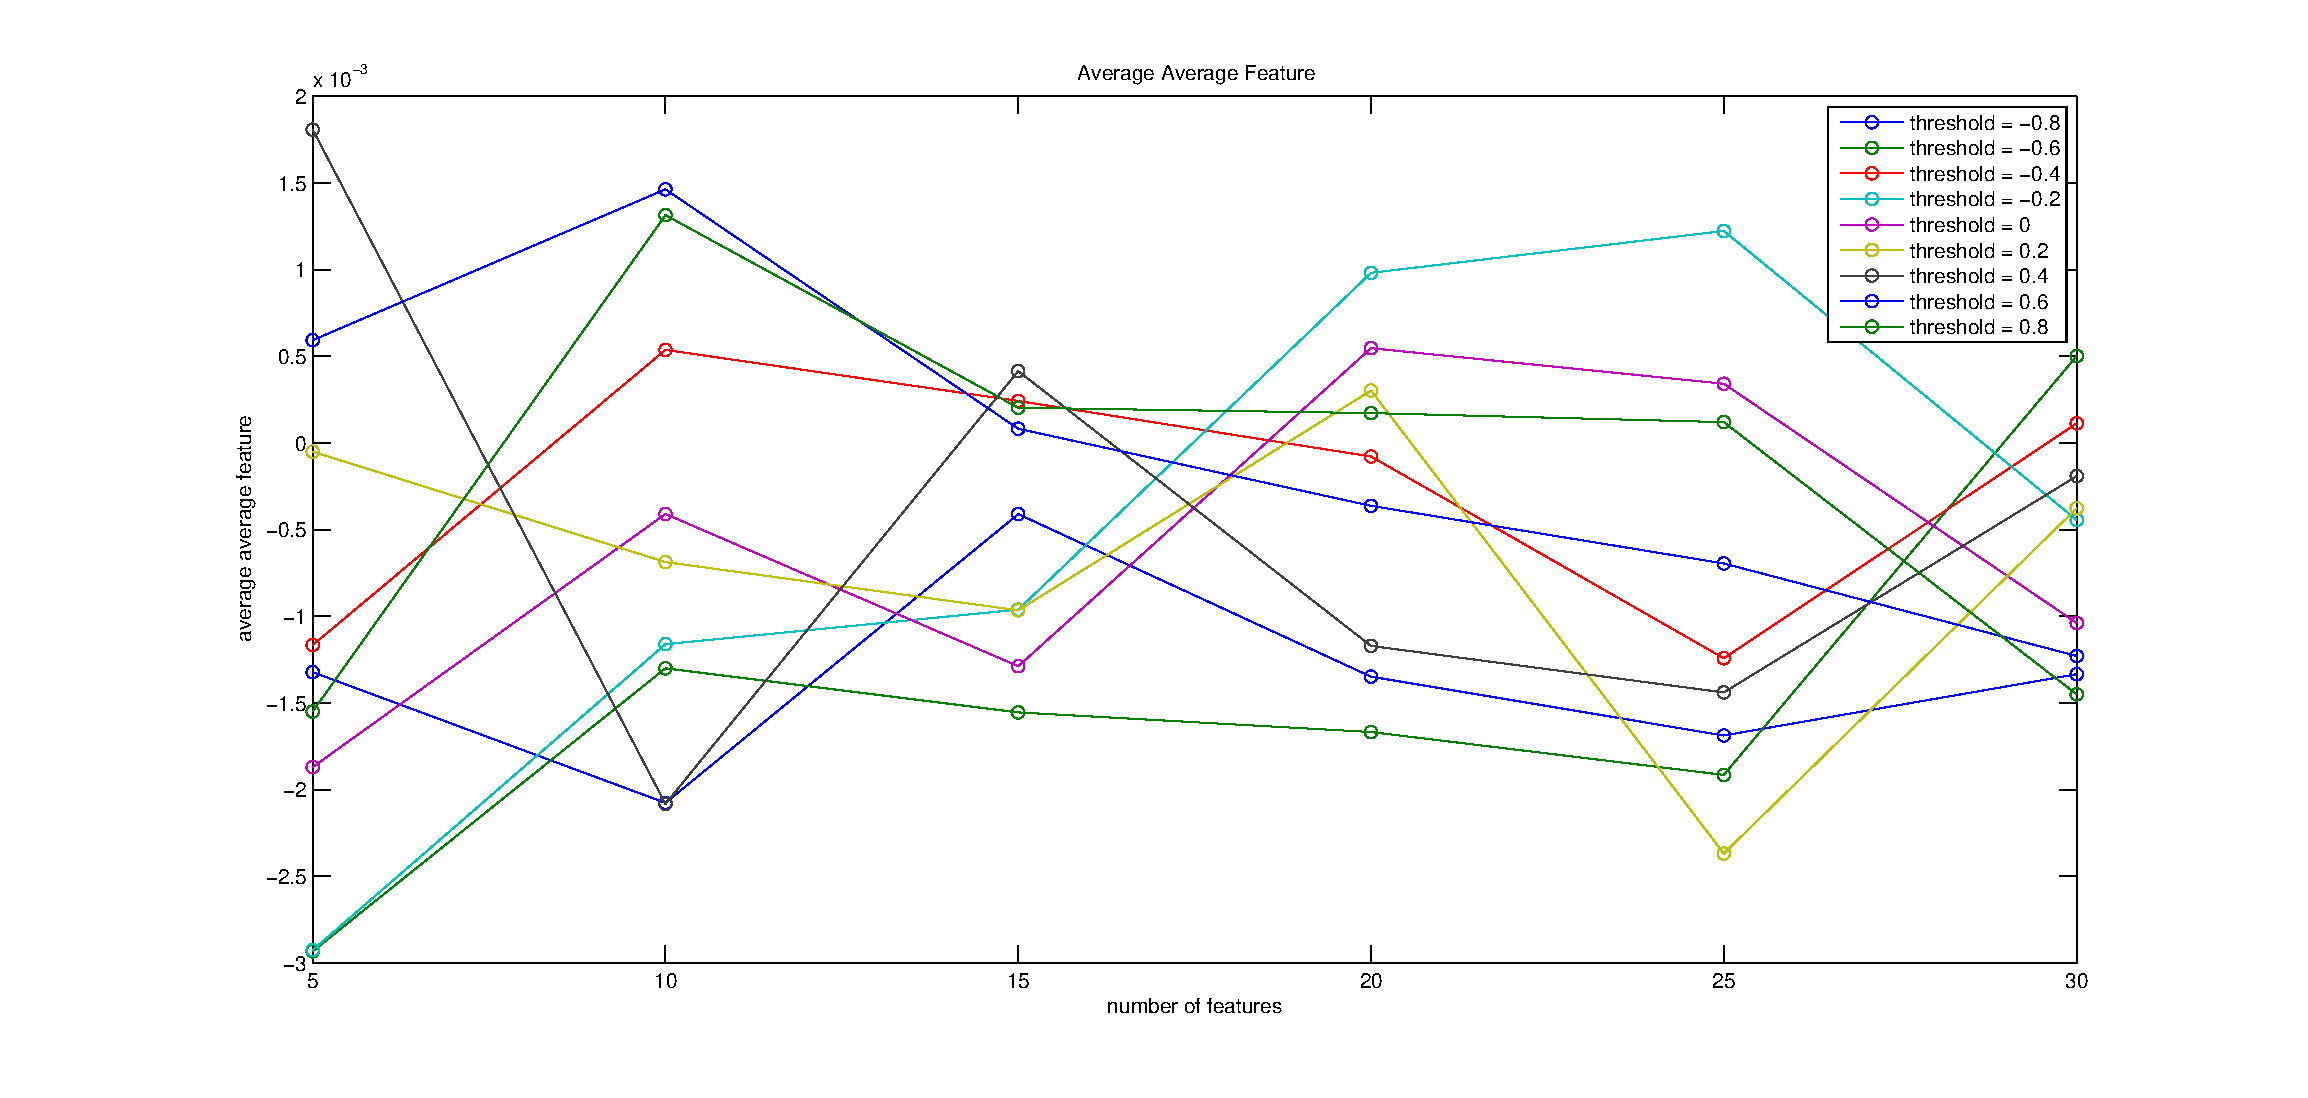
\includegraphics[width=\textwidth]{AverageAverageFeatureFeatures.eps}
\end{center}
\caption{Feature media media al variare del numero di features, tenendo fissa la threshold}
\label{2.1.7}
\end{figure}

\begin{figure}[!ht]
\begin{center}
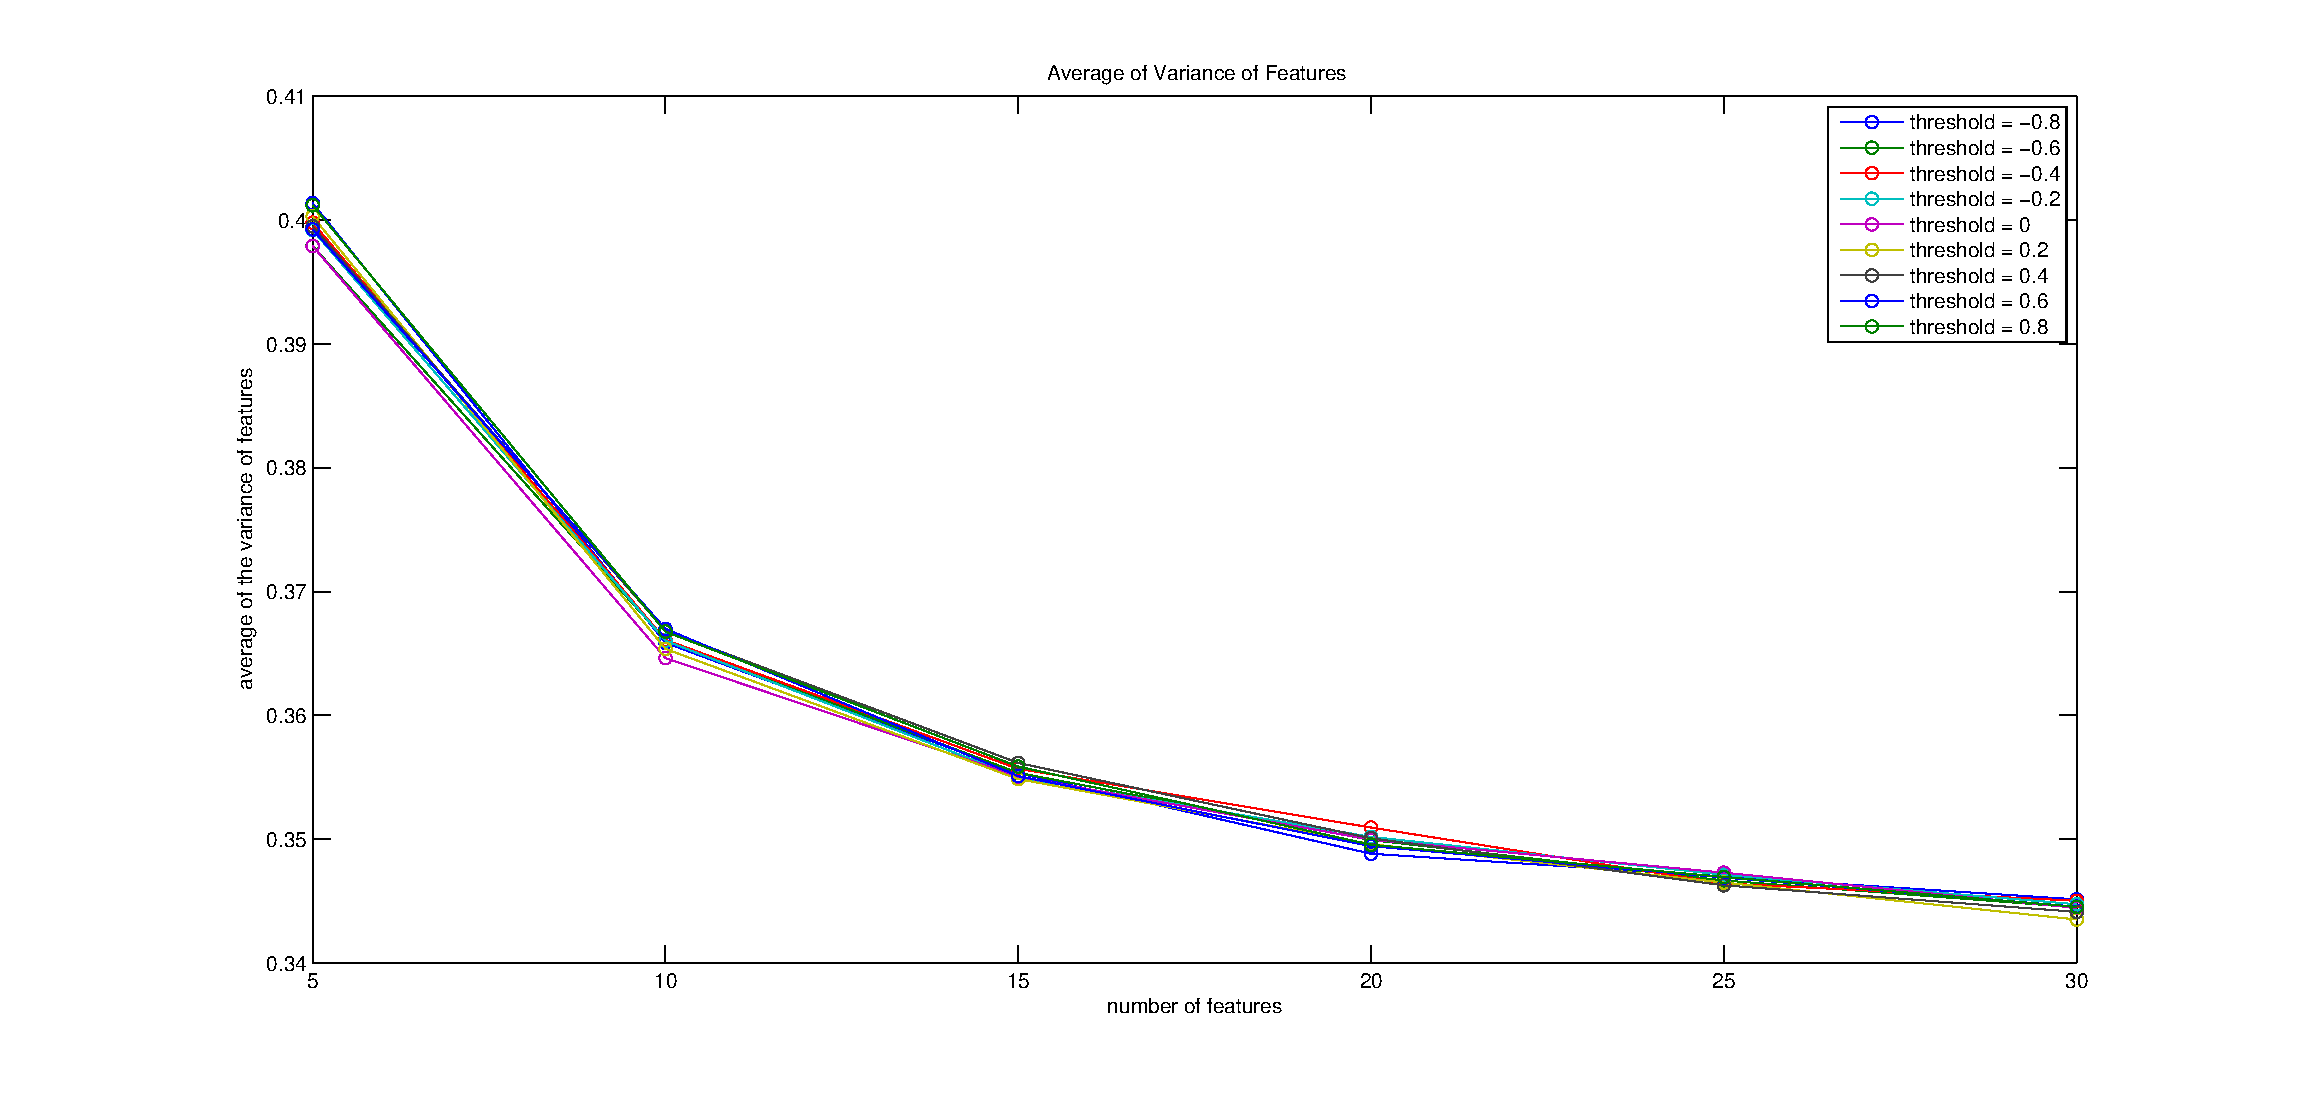
\includegraphics[width=\textwidth]{AveVarFeatFeatures.eps}
\end{center}
\caption{Varianza media delle features al variare del numero di features, tenendo fissa la threshold}
\label{2.1.8}
\end{figure}

In Figura~\ref{2.1.5} e ~\ref{2.1.6} sono riportati, rispettivamente, gli andamenti della media e della varianza medie delle features, al variare della threshold e con fissato numero di features.
In Figura~\ref{2.1.7} e ~\ref{2.1.8} sono invece riportati, rispettivamente, gli andamenti della media e della varianza medie delle features, al variare del numero di features e con threshold fissata.
\\Possiamo osservare che la media delle features \`{e} molto fluttuante in entrambi i casi, mentre la varianza resta circa costante al variare della threshold ma diminuisce all'aumentare del numero di features.
\\Queste misure ci forniscono dunque un'ulteriore conferma del fatto che il sistema dipende fortemente dal numero di feature, mentre non dipende in modo significativo dal valore della threshold. 

\subsection{Caso dinamico}

\section{Conclusioni}

\end{document}
